\documentclass{standalone}

\usepackage{tikz}
\usetikzlibrary{patterns}
\usetikzlibrary{arrows.meta}

\usetikzlibrary{decorations.markings}

\tikzset{
    midarrow/.style={
        decoration={markings, mark=at position 0.53 with {\arrow{Latex}}},
        postaction={decorate}
    }
}

\begin{document}

	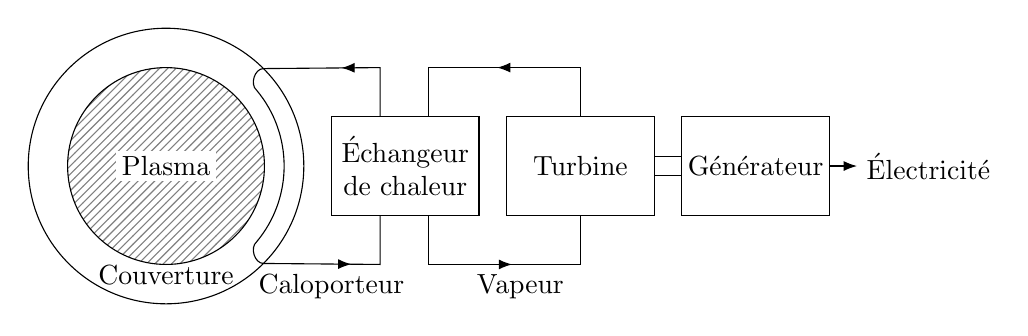
\begin{tikzpicture}
	
		\def\Rplasma{1.25}
		\def\Rblancket{1.75}
		
		\def\widthboxes{1.5*\Rplasma}
		\def\sepboxes{0.2*\Rblancket}
		\def\heightboxes{0.5*\Rplasma}
	
		\draw (0, 0) circle [ radius=\Rblancket cm ];
			
		\fill[pattern=north east lines, pattern color=gray] (0, 0)circle [ radius=\Rplasma cm ];
		
		\draw (0, 0) circle [ radius=\Rplasma cm ];
		
		\node[fill=white, text=black, inner sep=2pt] at (0,0) {Plasma};
		
		\node[ anchor=center ] at (0,-0.9*\Rblancket/2-0.95*\Rplasma/2) {Couverture};
		
		\def\Angle{45}
		
		\draw[ midarrow ] (\Rblancket + 1*\sepboxes + 0.33 * \widthboxes, \heightboxes) -- (\Rblancket + 1*\sepboxes + 0.33 * \widthboxes, \Rplasma) -- (\Angle:\Rblancket);
		
		\draw[ midarrow ] (-\Angle:\Rblancket) -- (\Rblancket + 1*\sepboxes + 0.33 * \widthboxes, -\Rplasma) -- (\Rblancket + 1*\sepboxes + 0.33 * \widthboxes, -\heightboxes);
		
		\def\angle{40}
		\draw (\angle:\Rblancket/2 + \Rplasma/2) to[ out=-\angle+180, in= 180] (\Angle:\Rblancket);
		
		\draw (\angle:\Rblancket/2 + \Rplasma/2)
      arc [
        start angle=\angle,
        end angle=-\angle,
        radius={\Rblancket/2 + \Rplasma/2}];
        
        \draw (-\angle:\Rblancket/2 + \Rplasma/2) to[ out=\angle+180, in= 180] (-\Angle:\Rblancket);
        
        \node[ anchor=north, align=center ] at (\Rblancket + 1*\sepboxes, -\Rplasma) {\shortstack{Caloporteur}};
		
		\draw
		(\Rblancket + 1*\sepboxes + 0 * \widthboxes, \heightboxes) -- 
		(\Rblancket +1 * \sepboxes+ 1*\widthboxes, \heightboxes) -- 
		(\Rblancket +1 * \sepboxes+ 1*\widthboxes, -\heightboxes) -- 
		(\Rblancket + 1 * \sepboxes + 0 * \widthboxes, -\heightboxes) -- cycle;
		
		\node at (\Rblancket + 1*\sepboxes + 0.5 * \widthboxes, 0) {\shortstack{Échangeur\\ de chaleur}};
		
		\draw[midarrow]
			(\Rblancket + 2*\sepboxes + 1.5*\widthboxes, \heightboxes) -- (\Rblancket + 2*\sepboxes + 1.5*\widthboxes, \Rplasma) -- (\Rblancket + 1*\sepboxes + 0.66*\widthboxes, \Rplasma) -- (\Rblancket + 1*\sepboxes + 0.66*\widthboxes, \heightboxes);
			
		\draw[midarrow]
			(\Rblancket + 1*\sepboxes + 0.66*\widthboxes, -\heightboxes) -- (\Rblancket + 1*\sepboxes + 0.66*\widthboxes, -\Rplasma) -- (\Rblancket + 2*\sepboxes + 1.5*\widthboxes, -\Rplasma) -- (\Rblancket + 2*\sepboxes + 1.5*\widthboxes, -\heightboxes);
			
		\node[ anchor=north, align=center ] at (\Rblancket + 2.5*\sepboxes + 1 * \widthboxes, -\Rplasma) {\shortstack{Vapeur}};
		
		\draw
		(\Rblancket + 2*\sepboxes + 1*\widthboxes, \heightboxes) -- 
		(\Rblancket +2*\sepboxes + 2*\widthboxes, \heightboxes) -- 
		(\Rblancket +2*\sepboxes + 2*\widthboxes, -\heightboxes) -- 
		(\Rblancket + 2*\sepboxes + 1*\widthboxes, -\heightboxes) -- cycle;
		
		\node at (\Rblancket + 2*\sepboxes + 1.5 * \widthboxes, 0) {\shortstack{Turbine}};
		
		\draw (\Rblancket +2*\sepboxes + 2*\widthboxes, 0.2*\heightboxes) -- (\Rblancket +3*\sepboxes + 2*\widthboxes, 0.2*\heightboxes);
		
		\draw (\Rblancket +2*\sepboxes + 2*\widthboxes, -0.2*\heightboxes) -- (\Rblancket +3*\sepboxes + 2*\widthboxes, -0.2*\heightboxes);
		
		\draw
		(\Rblancket + 3*\sepboxes + 2*\widthboxes, \heightboxes) -- 
		(\Rblancket +3*\sepboxes + 3*\widthboxes, \heightboxes) -- 
		(\Rblancket +3*\sepboxes + 3*\widthboxes, -\heightboxes) -- 
		(\Rblancket + 3*\sepboxes + 2*\widthboxes, -\heightboxes) -- cycle;
		
		\node at (\Rblancket + 3*\sepboxes + 2.5 * \widthboxes, 0) {\shortstack{Générateur}};
		
		\draw[ -{Latex} ] (\Rblancket +3*\sepboxes + 3*\widthboxes, 0) --  (\Rblancket +4*\sepboxes + 3*\widthboxes, 0);
		
		\node[ anchor=west, align=center ] at (\Rblancket + 4*\sepboxes + 3 * \widthboxes, 0) {\shortstack{Électricité}};
	
	\end{tikzpicture}

\end{document}